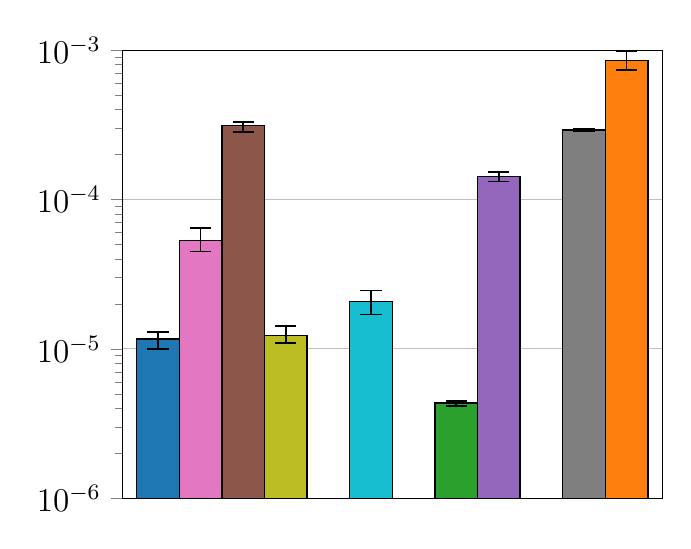
\begin{tikzpicture}
\definecolor{darkgray}{RGB}{169,169,169}
\definecolor{darkorange25512714}{RGB}{255,127,14}
\definecolor{darkslategray38}{RGB}{38,38,38}
\definecolor{darkturquoise23190207}{RGB}{23,190,207}
\definecolor{gray127}{RGB}{127,127,127}
\definecolor{lightgray204}{RGB}{204,204,204}
\definecolor{mediumpurple148103189}{RGB}{148,103,189}
\definecolor{orchid227119194}{RGB}{227,119,194}
\definecolor{sienna1408675}{RGB}{140,86,75}
\definecolor{steelblue31119180}{RGB}{31,119,180}
\definecolor{tabgreen}{RGB}{44,160,44}
\definecolor{tabolive}{RGB}{188,189,34}

\begin{semilogyaxis}[
  xmin=-0.5, xmax=7.1,
  xtick=\empty,
  ymin=1e-6, ymax=1e-3,
  ymajorgrids,
  ytick pos=left,
  tick align=outside,
  tick label style={font=\large},
]

% Group 1: PEACH/steelblue (0), pstnet/orchid (0.6), gnn_encoder/sienna (1.2), test_opt/olive (1.8)
\draw[fill=steelblue31119180, draw=black, line width=0.5pt] (axis cs:-0.3, 1e-6) rectangle (axis cs:0.3, 1.1675e-5);
\draw[fill=orchid227119194,   draw=black, line width=0.5pt] (axis cs:0.3,  1e-6) rectangle (axis cs:0.9, 5.3091e-5);
\draw[fill=sienna1408675,     draw=black, line width=0.5pt] (axis cs:0.9,  1e-6) rectangle (axis cs:1.5, 3.1270e-4);
\draw[fill=tabolive,          draw=black, line width=0.5pt] (axis cs:1.5,  1e-6) rectangle (axis cs:2.1, 1.2343e-5);

% Group 2: MaNGO/darkturquoise (3.0)
\draw[fill=darkturquoise23190207, draw=black, line width=0.5pt] (axis cs:2.7, 1e-6) rectangle (axis cs:3.3, 2.0718e-5);

% Group 3: Oracle/tabgreen (4.2), Oracle MGN/mediumpurple (4.8)
\draw[fill=tabgreen,              draw=black, line width=0.5pt] (axis cs:3.9, 1e-6) rectangle (axis cs:4.5, 4.3457e-6);
\draw[fill=mediumpurple148103189, draw=black, line width=0.5pt] (axis cs:4.5, 1e-6) rectangle (axis cs:5.1, 1.4253e-4);

% Group 4: No Context/gray (6.0), No Context MGN/darkorange (6.6)
\draw[fill=gray127,            draw=black, line width=0.5pt] (axis cs:5.7, 1e-6) rectangle (axis cs:6.3, 2.9218e-4);
\draw[fill=darkorange25512714, draw=black, line width=0.5pt] (axis cs:6.3, 1e-6) rectangle (axis cs:6.9, 8.5081e-4);

% Error bars
% steelblue/PEACH (center 0)
\draw[black, semithick] (axis cs:0,    1.0020e-5) -- (axis cs:0,    1.2944e-5);
\draw[black, semithick] (axis cs:-0.15,1.0020e-5) -- (axis cs:0.15, 1.0020e-5);
\draw[black, semithick] (axis cs:-0.15,1.2944e-5) -- (axis cs:0.15, 1.2944e-5);
% orchid/pstnet (center 0.6)
\draw[black, semithick] (axis cs:0.6,  4.4918e-5) -- (axis cs:0.6,  6.4341e-5);
\draw[black, semithick] (axis cs:0.45, 4.4918e-5) -- (axis cs:0.75, 4.4918e-5);
\draw[black, semithick] (axis cs:0.45, 6.4341e-5) -- (axis cs:0.75, 6.4341e-5);
% sienna/gnn_encoder (center 1.2)
\draw[black, semithick] (axis cs:1.2,  2.8242e-4) -- (axis cs:1.2,  3.3119e-4);
\draw[black, semithick] (axis cs:1.05, 2.8242e-4) -- (axis cs:1.35, 2.8242e-4);
\draw[black, semithick] (axis cs:1.05, 3.3119e-4) -- (axis cs:1.35, 3.3119e-4);
% olive/test_opt (center 1.8)
\draw[black, semithick] (axis cs:1.8,  1.1000e-5) -- (axis cs:1.8,  1.4248e-5);
\draw[black, semithick] (axis cs:1.65, 1.1000e-5) -- (axis cs:1.95, 1.1000e-5);
\draw[black, semithick] (axis cs:1.65, 1.4248e-5) -- (axis cs:1.95, 1.4248e-5);
% darkturquoise/MaNGO (center 3.0)
\draw[black, semithick] (axis cs:3.0,  1.7016e-5) -- (axis cs:3.0,  2.4613e-5);
\draw[black, semithick] (axis cs:2.85, 1.7016e-5) -- (axis cs:3.15, 1.7016e-5);
\draw[black, semithick] (axis cs:2.85, 2.4613e-5) -- (axis cs:3.15, 2.4613e-5);
% tabgreen/oracle (center 4.2)
\draw[black, semithick] (axis cs:4.2,  4.1519e-6) -- (axis cs:4.2,  4.4844e-6);
\draw[black, semithick] (axis cs:4.05, 4.1519e-6) -- (axis cs:4.35, 4.1519e-6);
\draw[black, semithick] (axis cs:4.05, 4.4844e-6) -- (axis cs:4.35, 4.4844e-6);
% mediumpurple/mgn_oracle (center 4.8)
\draw[black, semithick] (axis cs:4.8,  1.3208e-4) -- (axis cs:4.8,  1.5335e-4);
\draw[black, semithick] (axis cs:4.65, 1.3208e-4) -- (axis cs:4.95, 1.3208e-4);
\draw[black, semithick] (axis cs:4.65, 1.5335e-4) -- (axis cs:4.95, 1.5335e-4);
% gray/No Context (center 6.0)
\draw[black, semithick] (axis cs:6.0,  2.8797e-4) -- (axis cs:6.0,  2.9636e-4);
\draw[black, semithick] (axis cs:5.85, 2.8797e-4) -- (axis cs:6.15, 2.8797e-4);
\draw[black, semithick] (axis cs:5.85, 2.9636e-4) -- (axis cs:6.15, 2.9636e-4);
% darkorange/No Context MGN (center 6.6)
\draw[black, semithick] (axis cs:6.6,  7.3378e-4) -- (axis cs:6.6,  9.8727e-4);
\draw[black, semithick] (axis cs:6.45, 7.3378e-4) -- (axis cs:6.75, 7.3378e-4);
\draw[black, semithick] (axis cs:6.45, 9.8727e-4) -- (axis cs:6.75, 9.8727e-4);

\end{semilogyaxis}
\end{tikzpicture}